\documentclass[a4paper,twoside]{article}
 
\usepackage{subfigure} \usepackage{calc} \usepackage{amssymb}
\usepackage{amstext} \usepackage{amsmath} \usepackage{multicol}
\usepackage{pslatex} \usepackage{apalike} \usepackage{fancyhdr}
\usepackage{scitepress} \usepackage[small]{caption} \usepackage{url}
\usepackage{graphicx}

\begin{document} \onecolumn \maketitle \normalsize \vfill
 
\section{\uppercase{Introduction}} \label{sec:introduction} \noindent Spiegel
is a visualization system that was developed to process and visualize large
multidimensional data from simulations of galactic events such as black-hole
mergers, event horizons, and gravity waves~\cite{Bischof1:2010:Misc,Bischof06}.
Previous methods of user input for working with 3D models in the Spiegel
visualization framework were not intuitive. Ideally, we want astrophysicists
and other users to be able to view simulations in Spiegel in a simple and
natural way that allows them to see what is of interest to them. To accomplish
this goal we created NuWii, a system that captures the user's motions in 3D and
uses them to control the camera position in Spiegel. NuWii is designed to be
easily expandable to other applications that require 3D gesture input. Our
implementation uses a two level gesture hierarchy to accommodate custom gesture
input. We designed NuWii to be portable, easy to set up, and affordable. NuWii
uses two Nintendo Wii Remotes in stereo to capture the gesture input from the
user. We have also developed an algorithm to extract the 3D point from the two
images acquired by the Wii Remotes instead of using proprietary software (such
as the MATLAB Camera Calibration Toolbox) in order to keep the cost down for
anyone expanding upon our project. 
  
\section{\uppercase{Prior Work in the Field}} \noindent  A significant amount
of work has been done in the area of human-computer interaction, 3D point
recognition, and natural user interfaces. MIT created a 3D hand recognition
system in 2009 \cite{Wang09}. John Underkoffler is developing a 3D user
interface similar to the one seen in the movie Minority Report
\cite{Underkoffler10}. There has even been some previous experimentation with
3D interaction in Spiegel \cite{Bak04}. There have also been projects that use
Wii Remotes in other innovative ways. Eike Dehling did research on
stereo-vision algorithms with Wii Remotes \cite{Dehling08}. A group at the
University of Toronto investigated motion capturing with Wii Remotes
\cite{Wang08}. Johnny Lee experimented with reflective tape and Wii Remotes for
finger tracking  \cite{Lee08}. Most of the projects done with Wii Remotes use
MATLAB for camera calibration and resolving points in 3D space. However, using
MATLAB limits the audience, affordability, and flexibility of the software.
Some previous papers tracked multiple points in 3D, but did so only in the
context of head tracking. Head tracking limits the points range of motion
making it easier to correctly distinguish the points. Other projects had
minimal error checking involved [MY SECOND REFERENCE -JASON]. In contrast,
NuWii is able to track two points under more general conditions.
 
\section{\uppercase{Hardware}} \noindent The foundation of our hardware is the
Nintendo Wii Remote. We elected to use the Wii Remote for its affordability,
availability, and specialized camera hardware. In NuWii, the cameras on the
front of the Wii Remotes pick up infrared light reflected off the user's finger
tips. Two arrays of infrared LEDs supply the infrared light and finger slips
made from reflective tape reflect it back to the cameras.  We also machined a
wooden board to hold the Wii Remotes in place. The notches in our board hold
the Wii Remotes two feet apart and angled 22.5 degrees inward, but any
reasonable angle with overlapping fields of view could be used. All the
hardware used in NuWii is available to the average consumer living in a well
developed country. A photograph of the NuWii setup is shown in Figure 1.
 
\begin{figure}[h] \begin{center} 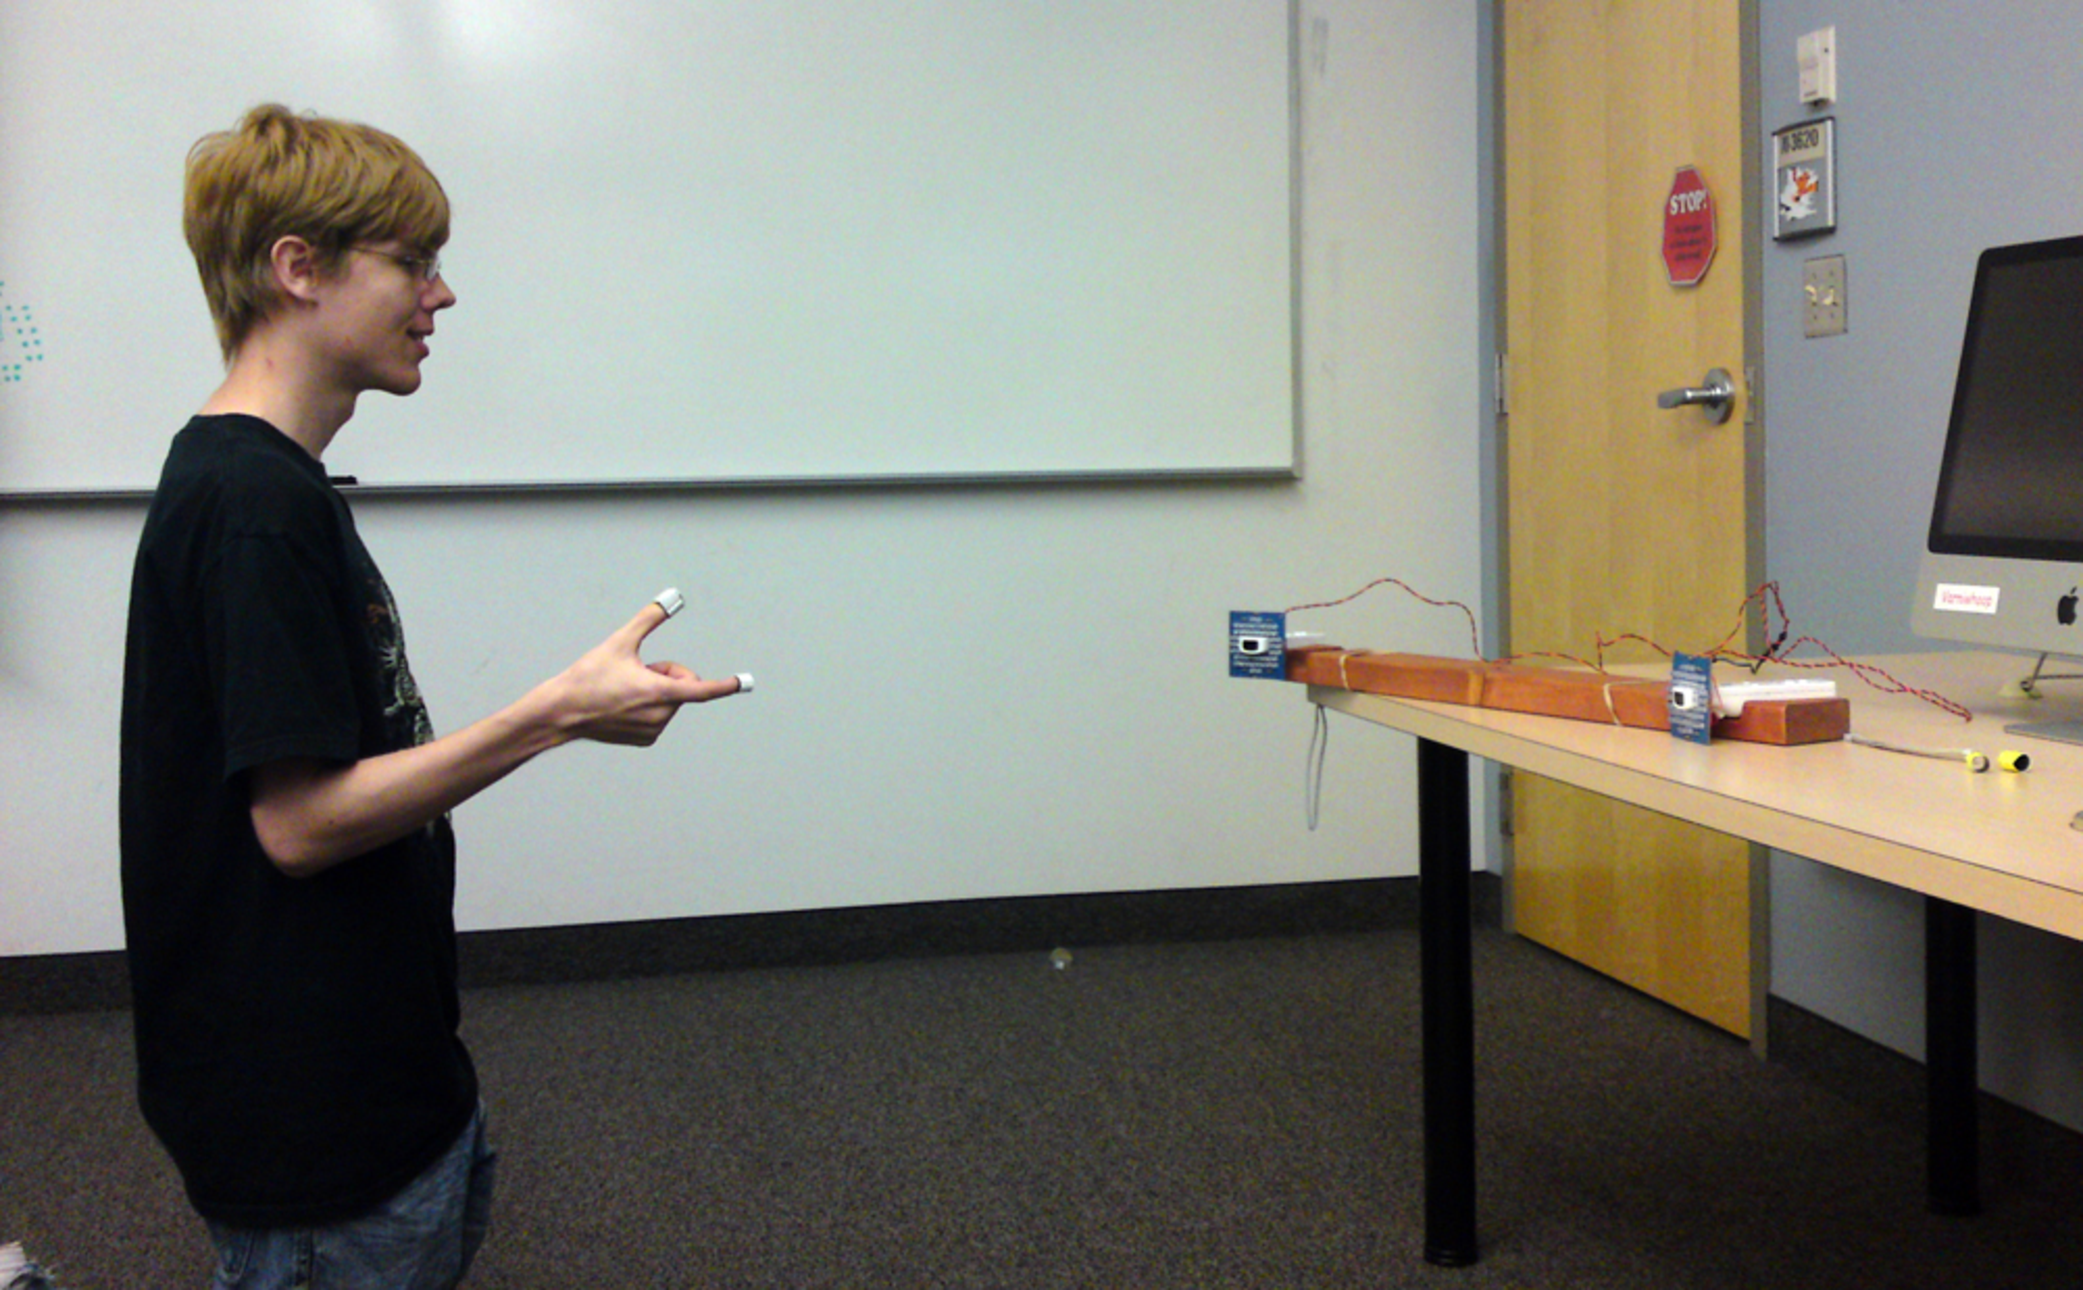
\includegraphics[width = 7.5cm]{setup}
\end{center} \caption{Photograph the NuWii setup. The user's gestures are being
tracked by the two infrared cameras.} \label{setup} \end{figure}
 
\subsection{The Wii Remote} The Wii Remote has a built-in 128x96 monochrome
camera. By using sub-pixel analysis, it is able to track up to four separate
points of infrared light and return their coordinates in a 1024x768 range
\cite{WiiBrew10}. This analysis of the image is done in hardware which makes
the output from the camera easy to deal with in software. The field of view of
the camera is 33.75 degrees vertical and 45 degrees horizontal. These values
can be derived from the resolution of the camera\cite{Lee08}. \\

The Wii Remotes use the Bluetooth HID protocol to communicate with their host.
However, they do not use the standard data types and are meant only to
communicate with a Wii gaming system. This lack of complete compliance makes
connecting the Wii Remotes to a computer somewhat complicated, but once the
connection has been made we have found it to be stable. Today, four years after
the release of the Wii, most of the functionality of the remotes is understood,
and a great number of libraries in a variety of high level languages have been
written to facilitate easier communication with the Wii Remotes and their
peripherals \cite{WiiBrew10}. We chose the \emph{motej} library because it is
open source, allowing us a greater understanding of how it communicates with
the Wii Remotes.  Additionally, both Spiegel and \emph{motej} are written in
Java making integration straightforward.

\subsection{Infrared LED Arrays} Each Wii Remote is surrounded with infrared
LEDs that supply light to be reflected back to the cameras. We made two arrays,
one for each Wii Remote, of 48 LEDs each. The wave length of the LEDs is 940 nm
which is the optimal wave length for the Wii Remotes' cameras \cite{WiiBrew10}.
The LEDs are arranged in eight groups wired in parallel. Each group contains 6
LEDs and a 75 Ohm resistor in series. The LED arrays are powered by a 12V, 1amp
power supply.
 
\subsection{Finger Slips} We created two finger slips out of reflective tape
that easily slide on and off the user's index finger and thumb
(Figure~\ref{fingerslips}). The finger slips completely cover the tips of the
user's fingers to ensure that the light from the LEDs is reflected back to the
cameras from any angle. We built the finger slips out of 3M 3000X Very High
Gain Reflective Tape. In order to hold the reflective tape together we used
small pieces of Nathan 3M Reflective tape. We also built finger slips
completely out of Nathan 3M Reflective tape. These finger slips seemed to work
just as well and were significantly less expensive than their high gain
counterparts. Nathan 3M Reflective tape is also more flexible which made it
easier to form the top of the finger slips.  

\begin{figure}[h] \begin{center}
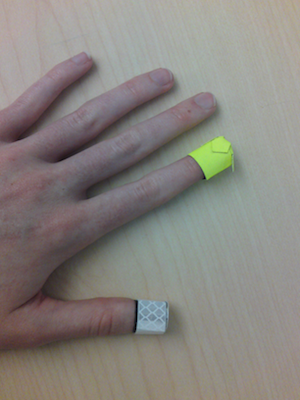
\includegraphics[width = 6cm]{fingerslips.png} \end{center} \caption{Finger
slips made of reflective tape.  Nathan 3M tape (index finger) and Very High
Gain tape (thumb).} \label{fingerslips} \end{figure}

\section{\uppercase{Stereo-Vision}}
\noindent In order to find a point's location in three dimensions, data from
two or more Wii Remotes must be combined. NuWii uses two Wii Remotes to find
points in 3D space. A third Wii Remote could be added to gain better accuracy,
but it would require a more advanced set up and increase the price of our
system. Our algorithm uses trigonometry to find the location in 3D space, given
the angle of the Wii Remotes and their distance apart.  

\subsection{Algorithm}
\noindent The algorithm takes input from two Wii Remotes. The output from the
Wii Remotes is in the form of (X,~Y) points in the range (0,~0) to (768,~1024).
The algorithm assumes that the Wii Remotes are in the same y and z plane and
are placed at known angles in the x plane. Deviating from the specified
orientation will produce errors/an error in the final result. It is possible to
get usable output from the algorithm without knowing the distance between the
Wii Remotes. However, if the distance is known then the .nal output will have
the same unit as the distance.  \\

\noindent Steps 1-3 are repeated for the input from both the left and right
cameras.  \newenvironment{indenteddescription} {\begin{list}{}{
\setlength{\labelwidth}{0pt} \setlength{\itemindent}{-37pt}
\setlength{\leftmargin}{37pt} \setlength{\listparindent}{\parindent}
\renewcommand{\makelabel}{\descriptionlabel} }} {\end{list}}

\begin{indenteddescription} \item[Step 1:]The range of the camera input is
altered to go from (-512, -384) to (512, 384). This is done by subtracting half
the maximum values for the respective axis (Figure~\ref{coordinates}). 

\begin{figure}[h] \begin{center} 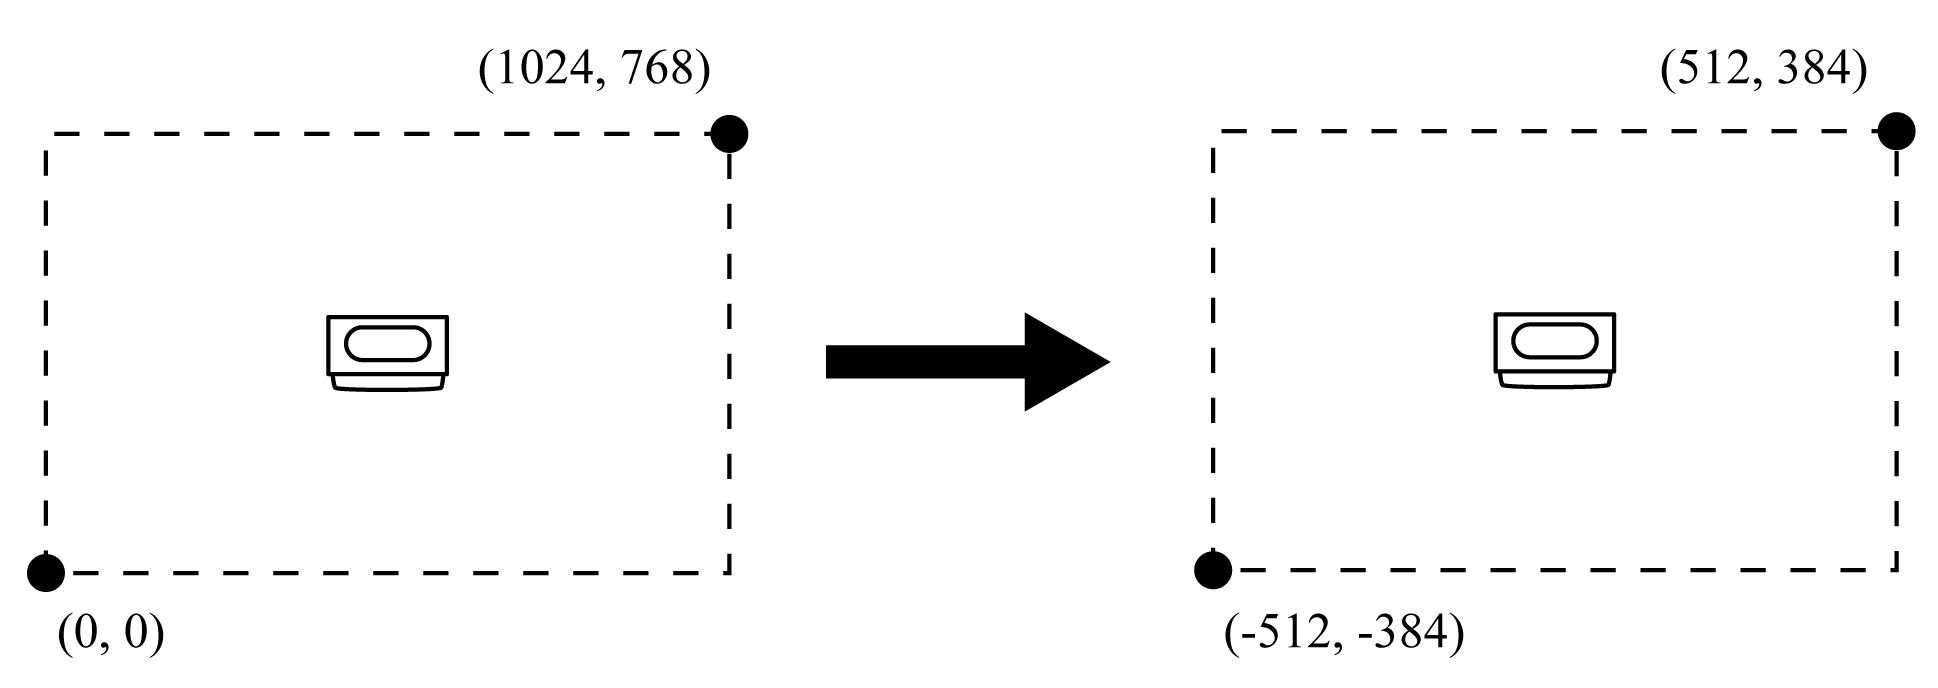
\includegraphics[width = 7.5
cm]{Diagram3_CoordinateShift.png} \end{center} \caption{Transforming the setup
coordinates.} \label{coordinates} \end{figure}

\item[Step 2:] Using the altered input, the points are normalized by dividing
the x value by 512, and the y value by 384. The x result is then multiplied by
half the horizontal field of view of the camera and the y result is multiplied
by half the vertical field of view in order to find the angles shown in
figures~\ref{topview} and~\ref{sideview}.  \begin{equation} \theta =
\frac{X}{512} \times \frac{45}{2} \end{equation} \begin{equation} \phi =
\frac{Y}{384} \times \frac{33.75}{2} \end{equation}


\begin{figure}[t] \begin{center} 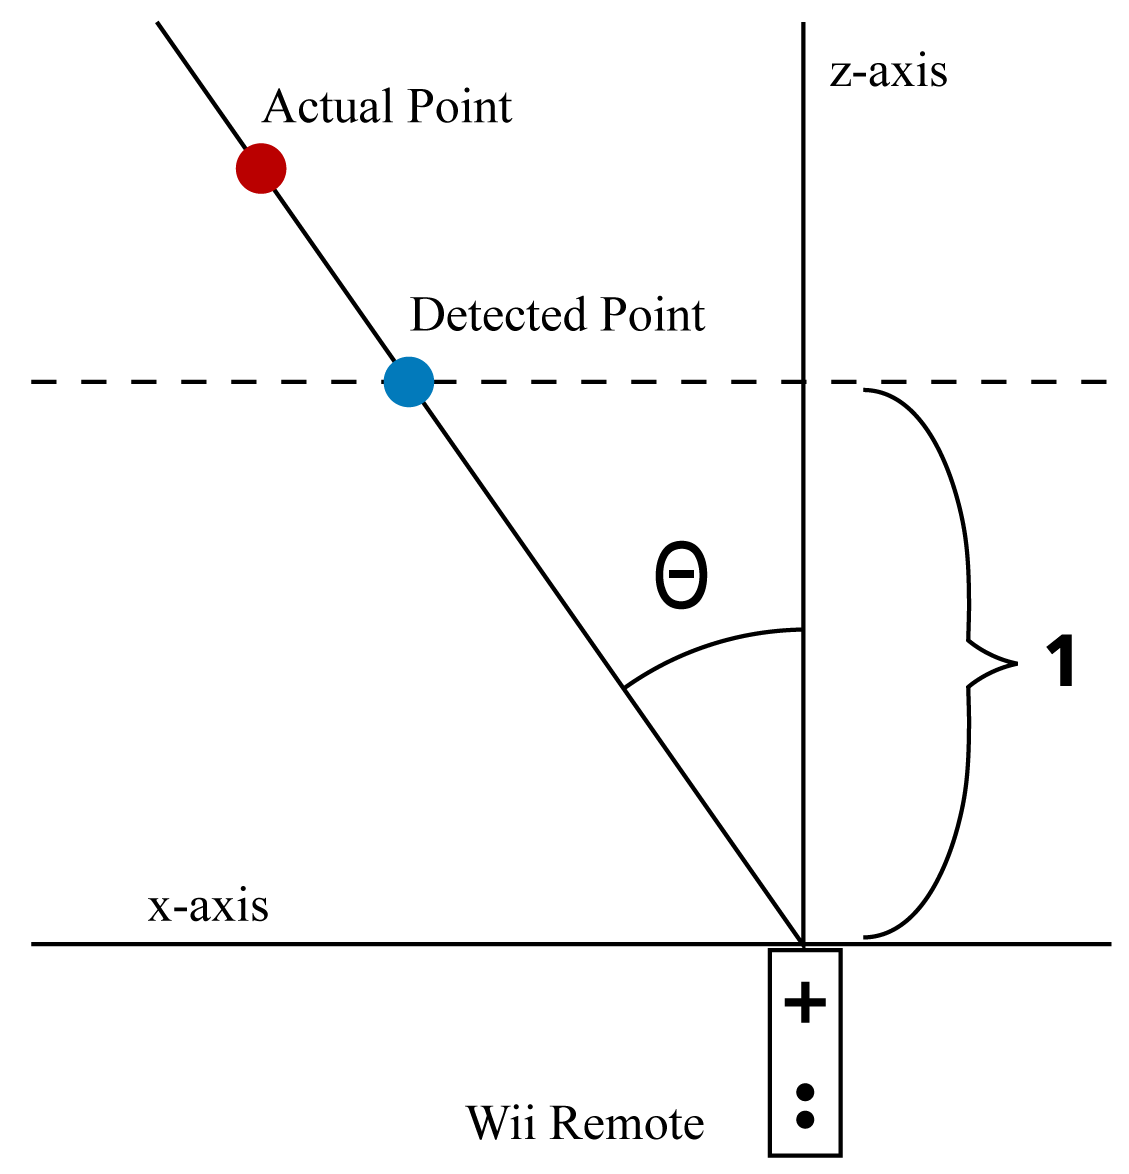
\includegraphics[height =
5cm]{Diagram1_CalcTopView.png} \end{center} \caption{Top View} \label{topview}
\end{figure}

\begin{figure}[t] \begin{center} 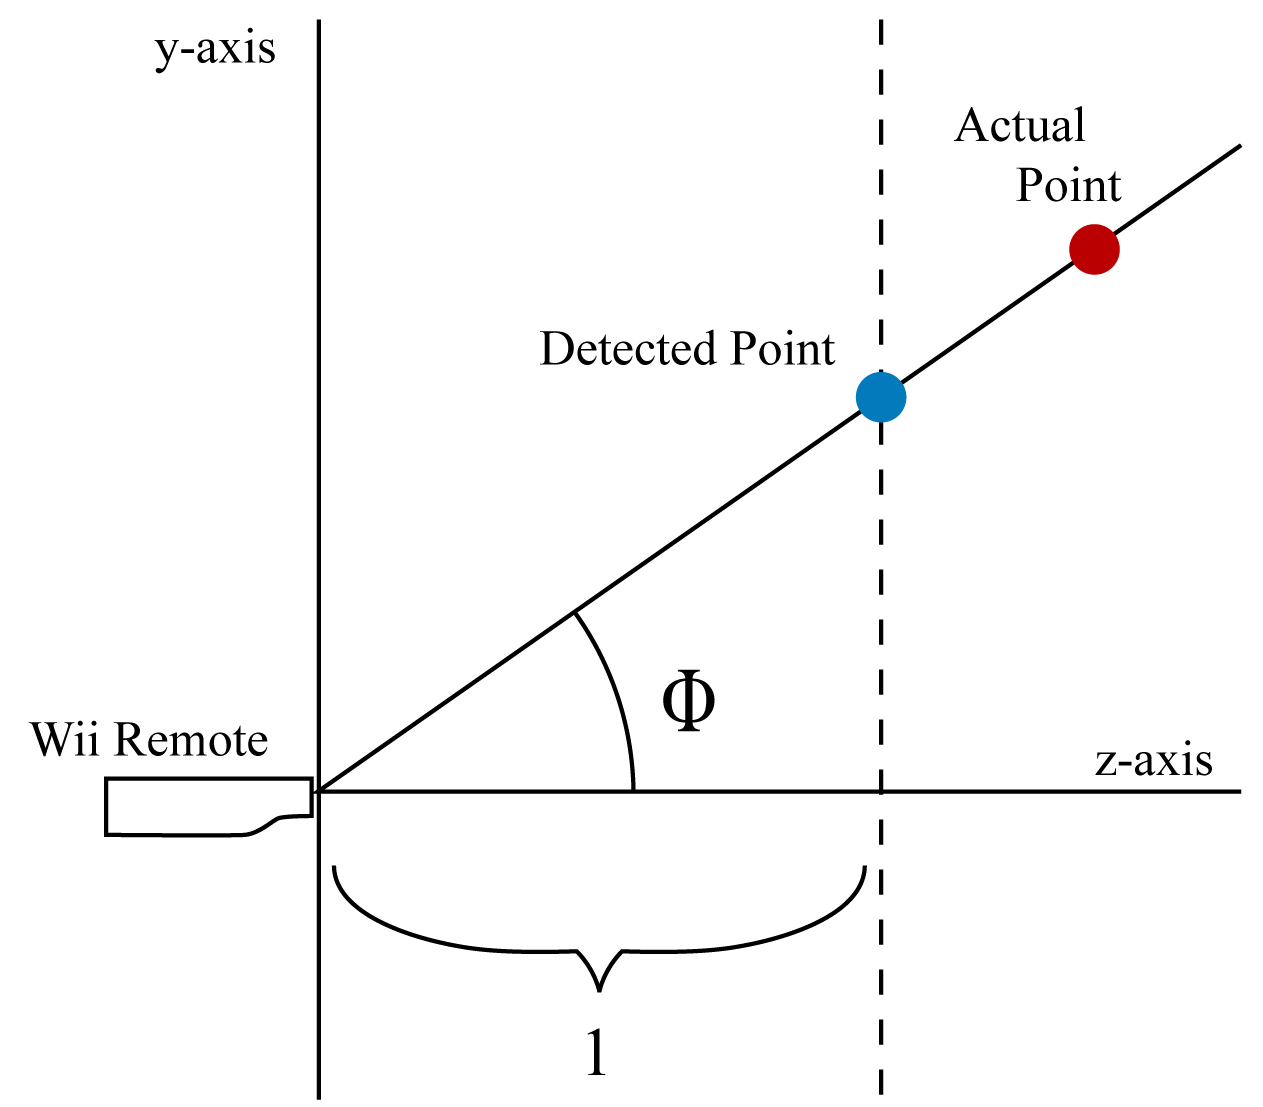
\includegraphics[height =
5cm]{Diagram2_CalcSideView.png} \end{center} \caption{Side View}
\label{sideview} \end{figure}

\item[Step 3:] Trigonometry is used to find a normalized point one unit away from
the cameras.  \begin{equation}\label{eq1} X' = tan(\theta) \end{equation}
\begin{equation}\label{eq2} Y' = tan(\phi)  \end{equation}
\begin{equation}\label{eq3} Z' = 1          \end{equation}

\item[Step 4:] After the normalized points are found, they are rotated by
alpha, the angle between the Wii Remotes and the y-z plane shown in
figure~\ref{finalpoint}. Rotating the points is not required if the Wii Remotes
are parallel. The following equations are used to rotate the points. 

\begin{flushleft} \begin{equation}\label{eq4} X' = X'cos(\alpha) + sin(\alpha)
\end{equation} \begin{equation}\label{eq5} Y' = Y'\end{equation}
\begin{equation}\label{eq6} Z' = -1 * X'sin(\alpha) + cos(\alpha)\end{equation}
\end{flushleft}


\item[Step 5:] The distance between the Wii Remotes is added to the x value of
the points from the right Wii Remote. (The right Wii Remote will be on the left
when looking into the cameras of the remotes. Imagine looking towards the user
from the camera's perspective). The units of the final output will be the same
as the units used to measure this distance. If the distance between the Wii
Remotes is unknown then 1 should be added instead.

\begin{equation}\label{eq7} X_{r}' = X_{r}' + d \end{equation}

This step moves the points read by the right camera into the correct coordinate
system in relation to the left camera.  \end{indenteddescription}

\begin{figure}[h] 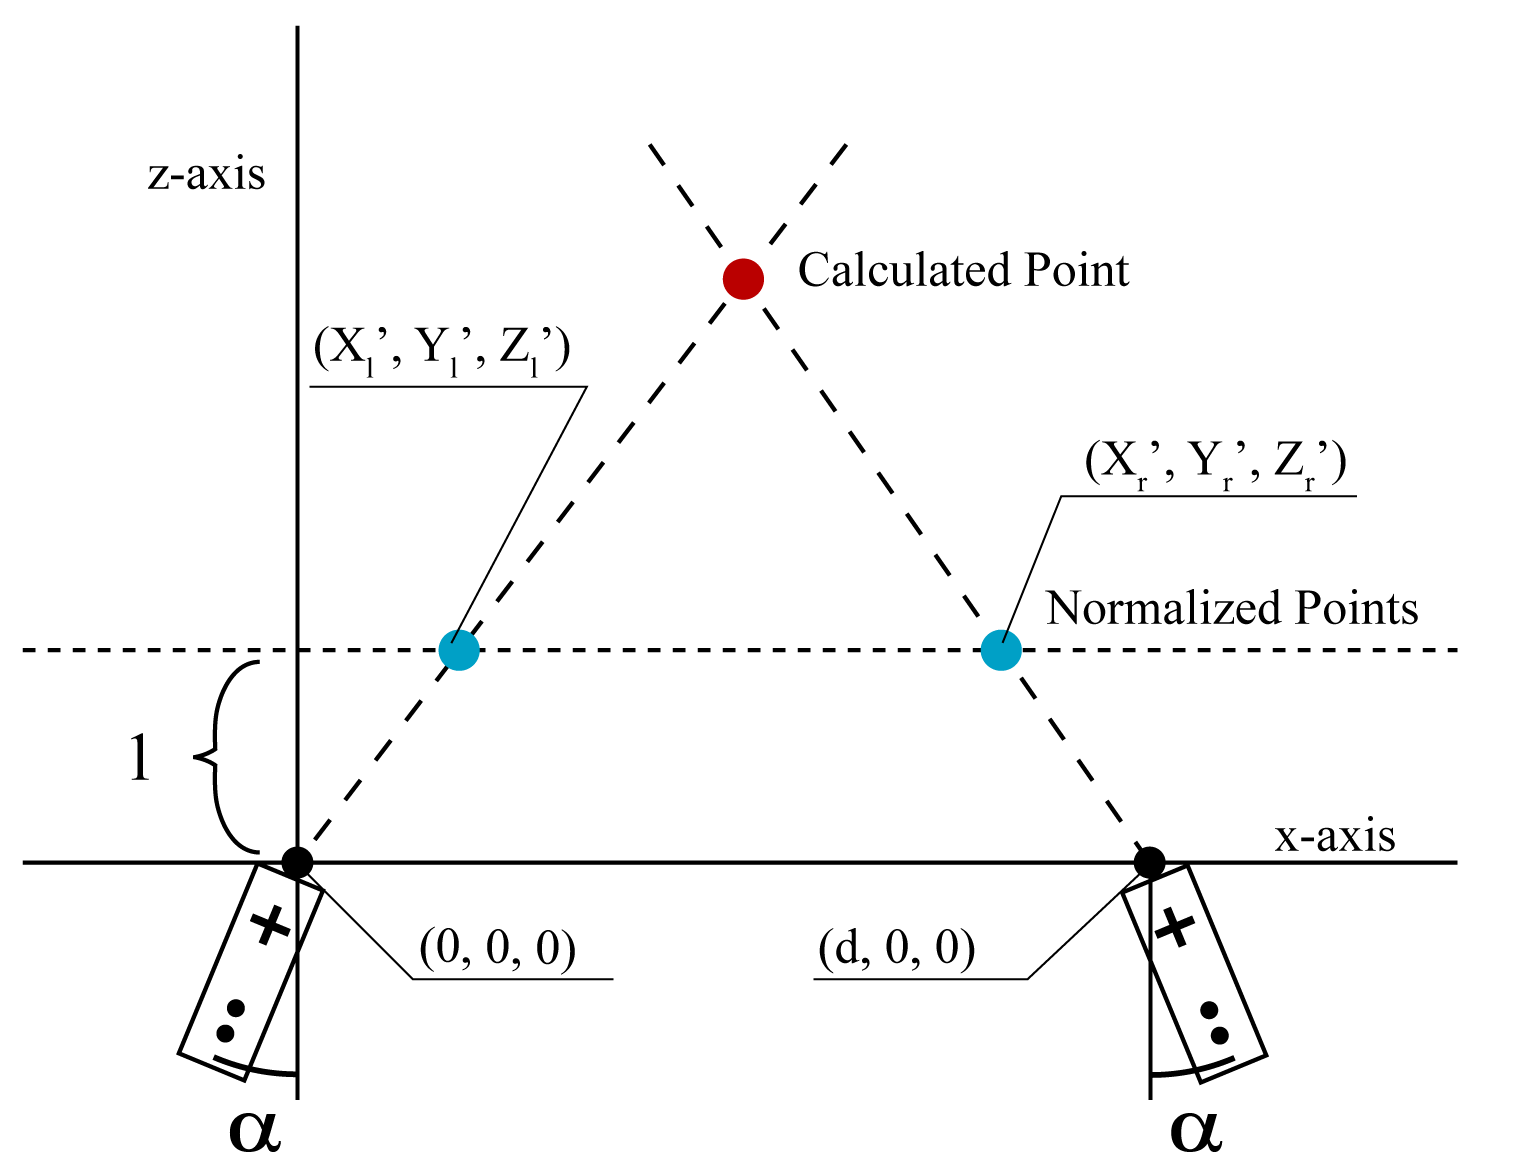
\includegraphics[width = 7.5cm]{Diagram4_FinalPoint.png}
\caption{Finding the 3D point.} \label{finalpoint} \end{figure}

Using the new points, rays can be created originating from the Wii Remotes and
going through the left and right calculated points accordingly.
Figure~\ref{finalpoint} shows that the left camera is at the origin (0,0,0) and
the right camera is at position (d,0,0) where d is the distance between the Wii
Remotes. A ray collision algorithm is used to find the location along the rays
where they are closest to colliding. This location is the approximate position
of the point. The exact location of the collision can not be calculated because
the rays will not collide perfectly due to error in the data captured by the
Wii Remotes. The distance between the two rays is used to evaluate error in the
calculation.

\subsection{Multiple Points}Aside from hardware and environmental issues, this
algorithm will always work when sensing one point. However, reading two points
introduces problem areas. These problems occurred most often when both points
lie in the same y plane. The problems occur because the Wii Remotes transmit
only the coordinates of the infrared points that they see. This means that
there are no surrounding visual aids to help distinguish between the two
points. Because of this limited information, it can be impossible to tell which
point from the second Wii Remote corresponds to the point seen by the first Wii
Remote in certain situations.  
 
\begin{figure}[ht] \begin{center}
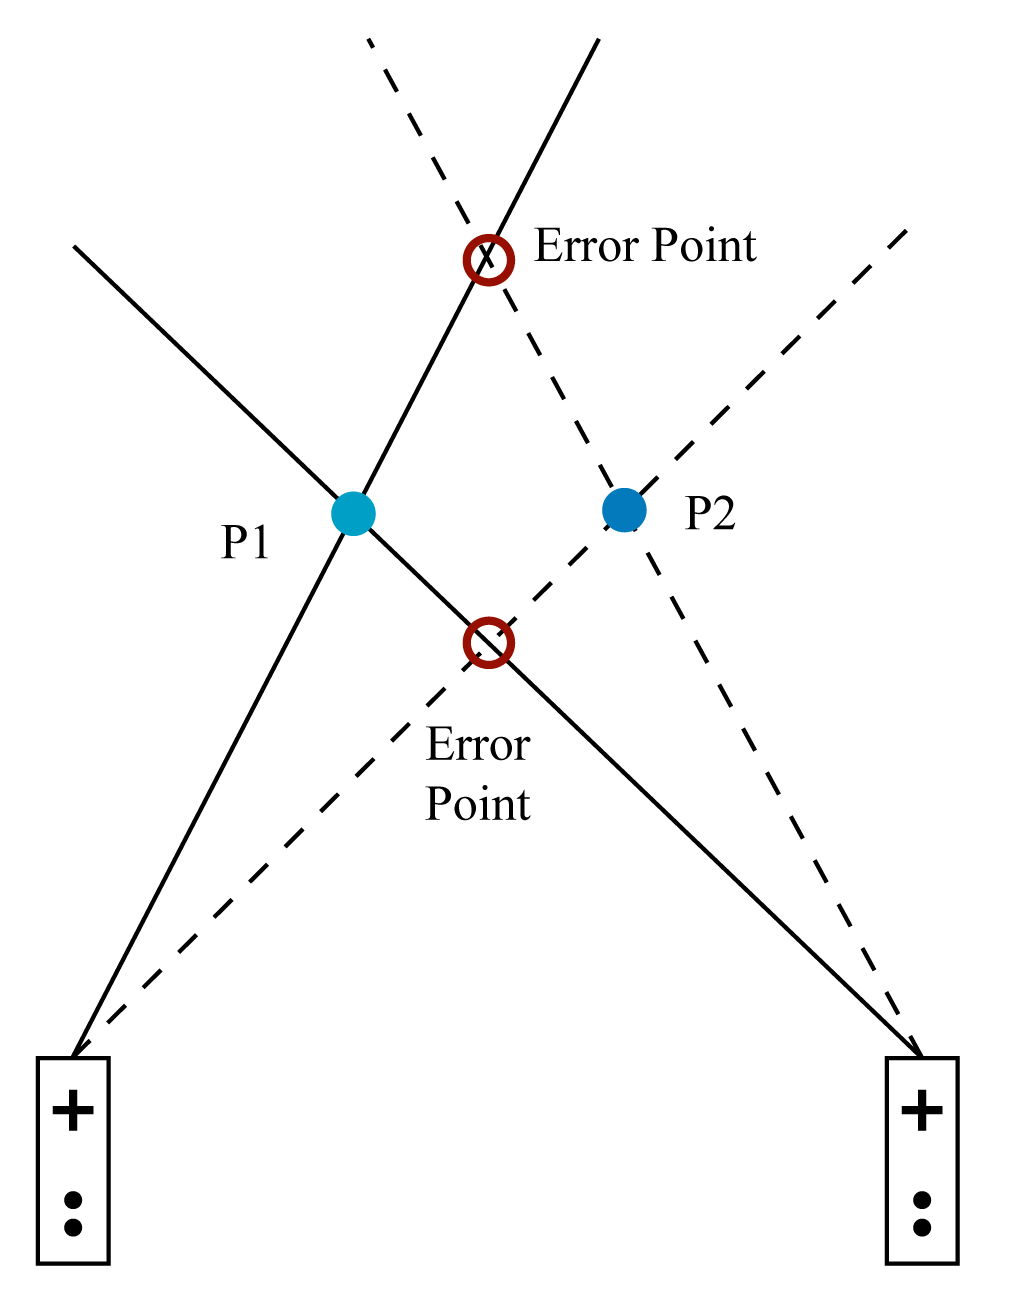
\includegraphics[height = 7.5cm]{Diagram5_IntersectingRays} \end{center}
\caption{Lines intersecting incorrectly.} \label{intersection} \end{figure}

When the points are not in the same y plane the ray collision  error can be
used to match the correct points. To distinguish between these points both
possibilities are tested and the pair with the smaller error is used. This
method does not work when the points are in the same y plane because both pairs
appear to be valid, as is made clear by figure~\ref{intersection}. More error
is eliminated by leveraging the knowledge that the leftmost point on the first
camera should be paired with the leftmost point on the second camera in most
situations. When we cannot distinguish the points using the above methods, we
remember that the Wii Remotes return the points that they detect in the same
order throughout a session, and assume that they have not changed. This can be
a problem if a camera stops sensing points and then flips the order it senses
them in. While there still exist some problems with multiple points, they
remain largely unnoticed because the points are constantly updating.

\begin{figure*}[ht] \begin{center}
\subfigure[Pinch]{\label{pinch}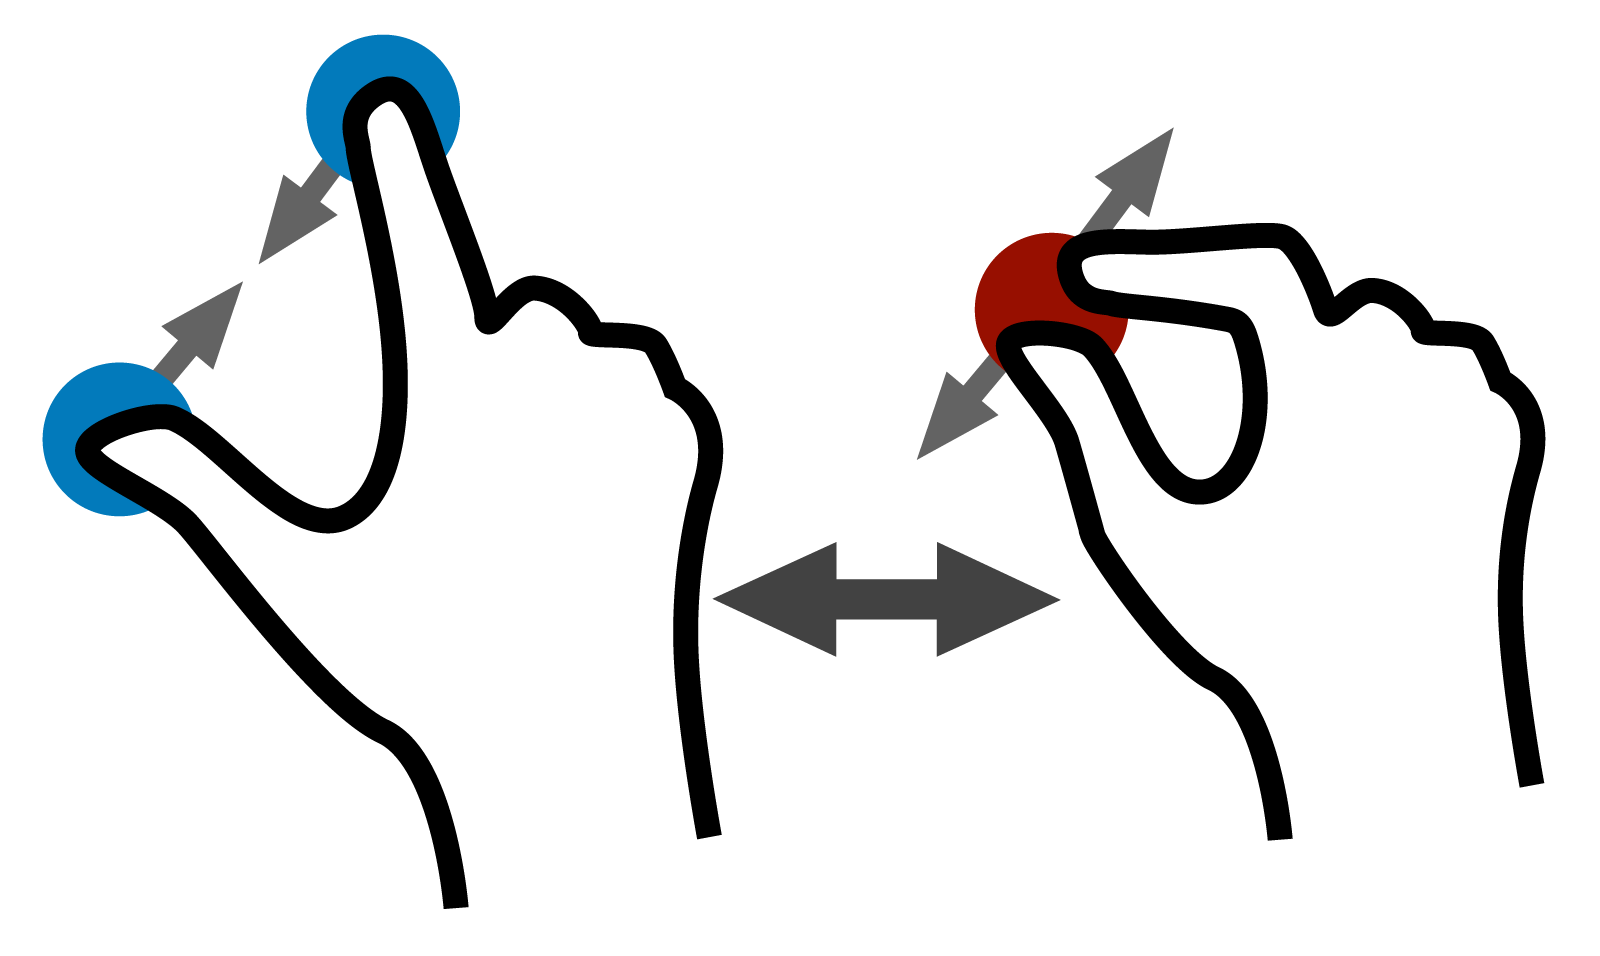
\includegraphics[width = 5cm]{Pinch.png}}
\subfigure[Swipe]{\label{swipe}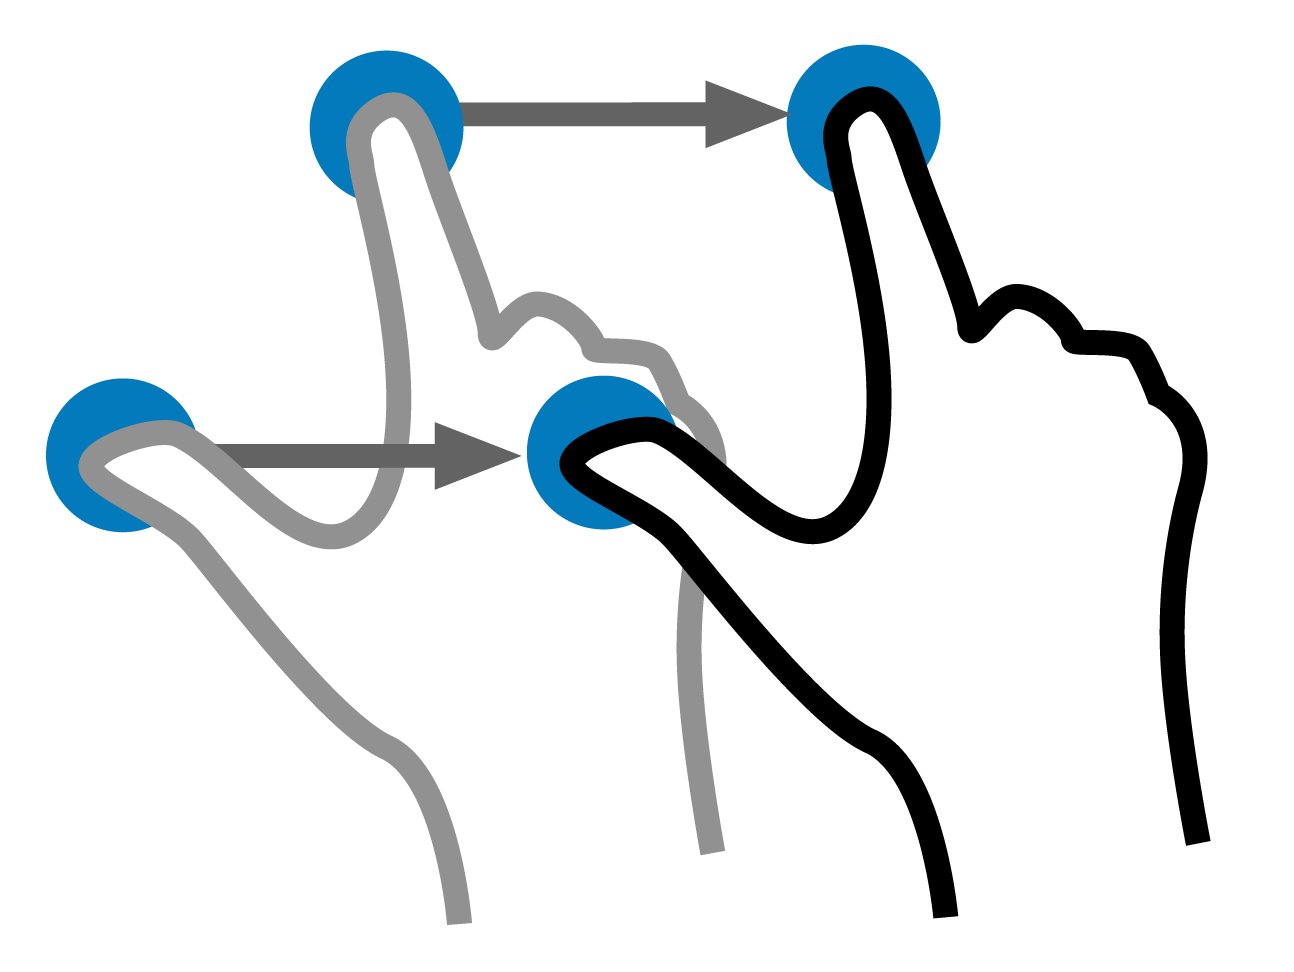
\includegraphics[width = 5cm]{Swipe.png}}
\subfigure[Rotate]{\label{rotation}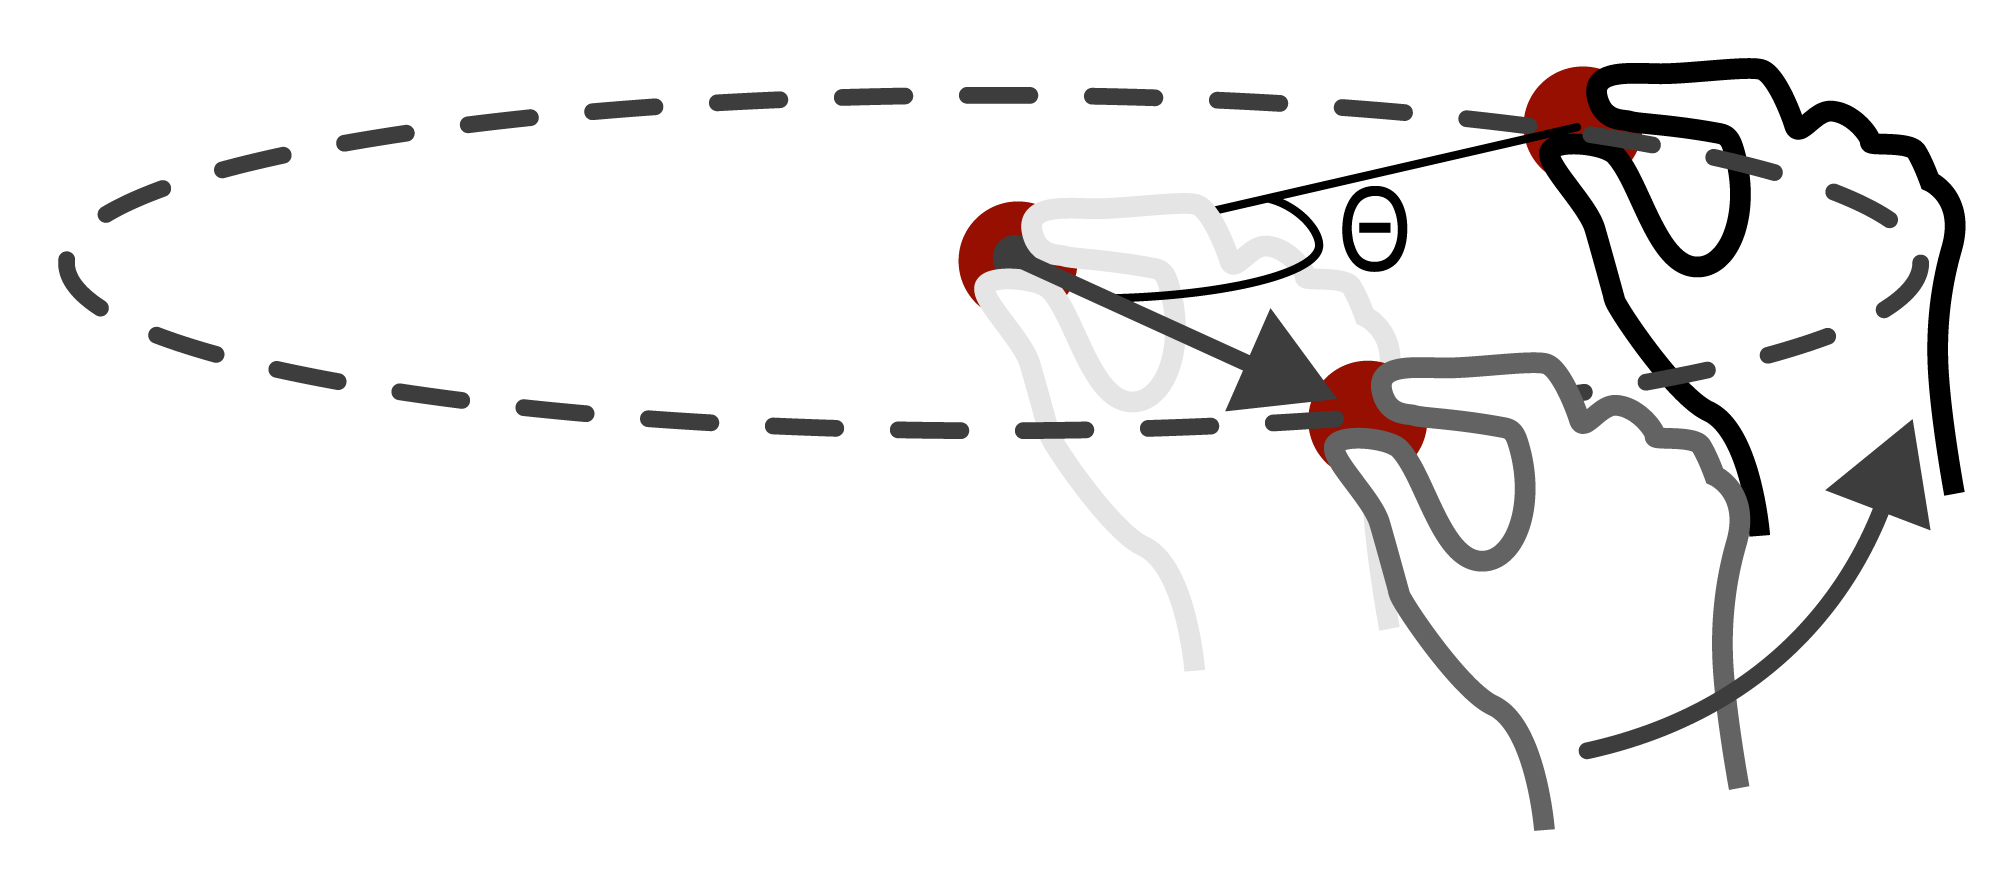
\includegraphics[width = 5cm]{Rotation.png}}
\end{center} \caption{Various Gestures.} \label{gestures} \end{figure*}

\section{\uppercase{Gestures}} Our implementation of gesture recognition is
designed to be easily expandable. This is accomplished by using two levels of
gestures: basic gestures and composite gestures. Basic gestures are simple
motions and movements of the users hands that are detected within our
stereo-vision algorithm. We created a gesture interface in Java that can be
implemented by any class that needs to detect these basic gestures. The second
level of gestures is composite gestures. Composite gestures are combinations of
basic gestures that can be used for more complex input. These higher-level
gestures are implemented by the class that uses our interface and are more
application specific than basic gestures.  \subsection{Basic Gestures} There
are two categories of basic gestures implemented at this time: pinch and swipe.
A pinch gesture (Figure~\ref{pinch}) is activated when the two points seen by
the cameras move close enough together that they appear to be one point. There
is also an unpinch gesture that is activated when a pinched point separates
back into two points. An unpinch gesture can only be detected after a pinch has
taken place, which keeps the cameras from falsely identifying two unrelated
points as an unpinch gesture. The other basic gesture, swipe, is activated when
the points move a set distance in any dimension (Figure~\ref{swipe}). The
movement of either one or two points is tracked depending on how many the
cameras see. Tracking any number of points allows swipe to be detected
regardless of the pinching state. Swipes can be detected in both positive and
negative directions in all three dimensions for a total of six different swipes
that can be detected and used for composite gestures.

\subsection{Composite Gestures} By combining the basic gestures discussed above
and the current position of the points, application specific gestures can be
created. These composite gestures can be very simple, using just one basic
gesture to activate some sort of onscreen movement, or as complicated as
necessary, making use of several gestures in sequence. A rather conventional
application would be to map the movement of the points to cursor position and
the pinch/unpinch to a click.  The gestures implemented for Spiegel, described
in detail in the following sections, provide an example of more complex
composite gestures. 

\section{\uppercase{NuWii and the Spiegel Visualization Framework}}
The Spiegel framework was developed to visualize large multidimensional
astrophysical data. It is designed according to the UNIX paradigm of pipes and
small utilities that do one thing and do it well~\cite{Bischof06}. These small
utilities are called "functions" by Spiegel developers. Once the Spiegel GUI is
loaded, the user chooses the functions that they want to use from the menu and
the functions appear on screen as boxes with incoming and outgoing arrows. For
example, in order to display a set of simulation data in 3D, the user would
import five boxes - one to import the data file from the file system, one that
extracts the stars from the data, one that converts the star data into a format
that Java3D can understand, one that determines camera parameters, and finally
a display window for the image. Our team wrote two new functions for Spiegel.
One of these, named WiimoteControl, connects the Wii Remotes and interprets the
data read from the Wii Remotes as camera coordinates. The other,
3DPointDisplay, shows the points from the Wii Remotes in 3D space and is used 
for debugging the system when it appears not to work.

 
\subsection{Camera Control in Spiegel} In the Spiegel visualization
framework, three composite gestures were implemented to control the camera
position. These gestures are used to enter different camera movement modes.
Each gesture starts with a pinch that is followed by a swipe. The pinch sets a
center point to be used as a reference for movement in each camera movement
mode. The direction of the swipe determines which mode is activated. The user
can easily exit each movement mode by unpinching their fingers. Using these
three gestures the user can view the simulation from any angle.

\subsection{Camera Orientation and Coordinates} The best way for the user to
remain oriented when viewing a simulation in Spiegel is to have the camera
constantly pointing towards the origin. The simplest way to achieve this
behavior is to use a spherical coordinate system for the camera position.
Changes in the inclination and azimuth angles correspond to vertical and
horizontal rotation respectively and changing the radial distance acts as a
zooming function. See Figure~\ref{camera}. In NuWii, each camera movement mode
changes the value of one of the spherical coordinates.

\begin{figure}[h] \begin{center} 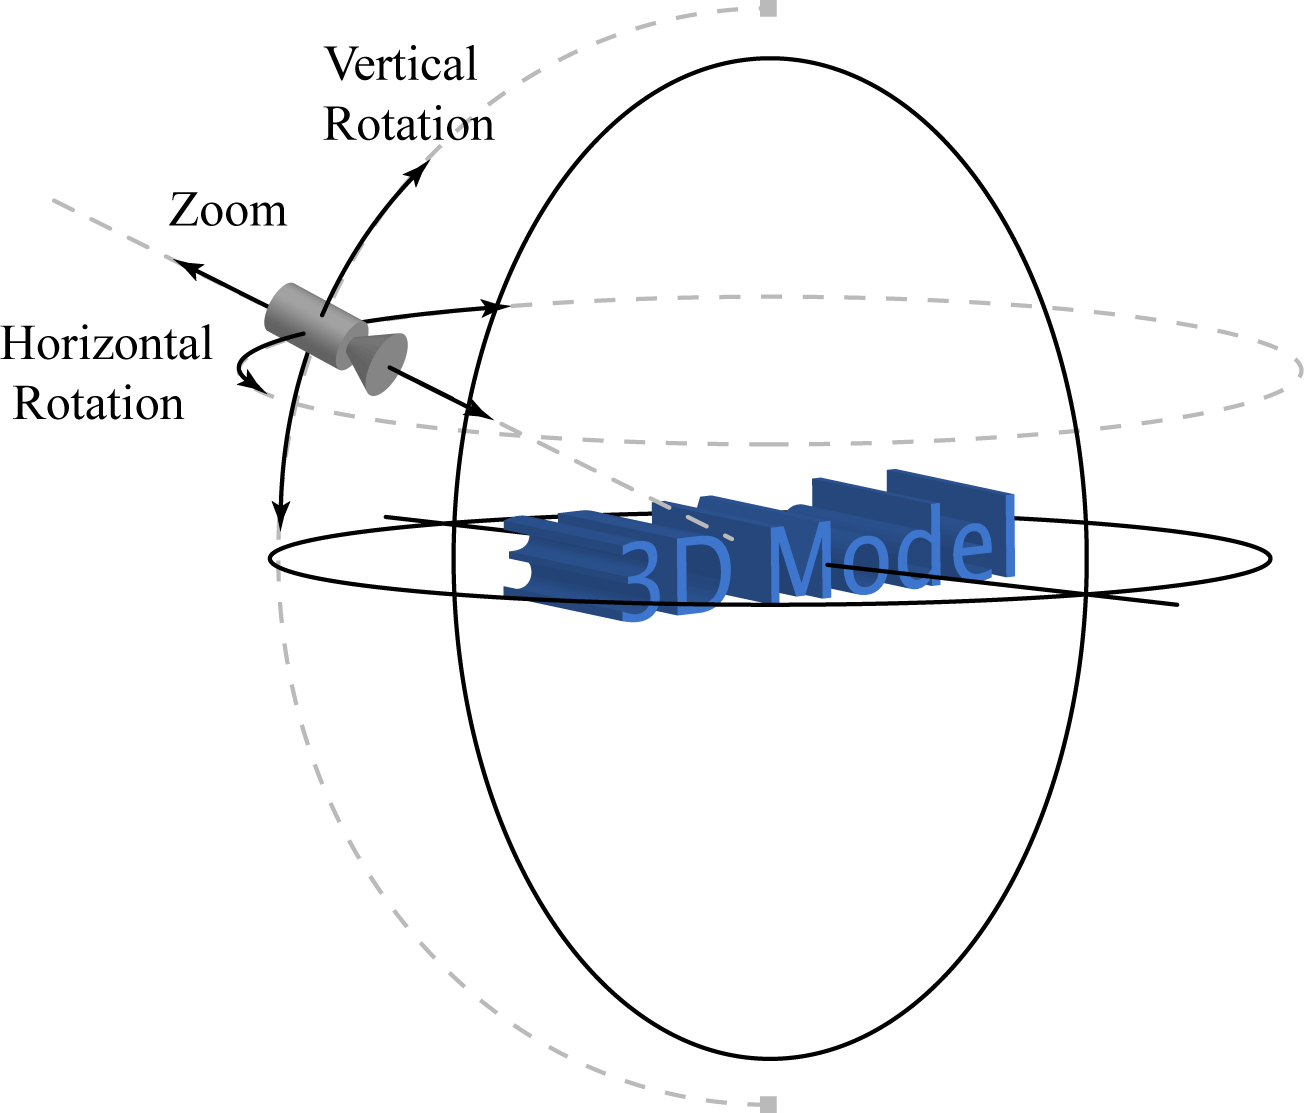
\includegraphics[width = 7.5cm]{Camera}
\end{center} \caption{Camera in relation to the scene} \label{camera}
\end{figure}


\subsection{Camera Movement Modes} There are three camera movement modes:
horizontal rotation, vertical rotation, and zoom. Horizontal rotation is
activated by pinching and swiping to the right. To rotate the model, the user
rotates the pinched point around the reference point to move the camera around
the model (Figure~\ref{rotation}). Swiping backwards (towards the user) after
pinching triggers vertical rotation mode. After swiping, the user can move
their hand up or down to rotate the camera vertically around the model.
Horizontally, the camera can be rotated around the model indefinitely, but
vertical rotation is capped at positive and negative 90 degrees. This cap keeps
the user from moving the camera over the model which would make the view
up-side-down. The zoom control is activated by pinching and then swiping down.
Once in the zoom mode, the distance between the center point and the current
point is used to scale the zoom speed. If the current point is at the center
point set by the pinch, then the camera will be stationary. When the current
point is in front of the center point, then the camera will zoom in. Similarly,
if the current point is behind the center point, then the camera will zoom out.

 
\section{\uppercase{Integrating with the Spiegel Visualization Framework}} 
\section{\uppercase{Conclusions and Future Work}} There is a lot of potential
for future expansion of NuWii. Right now, our program recognizes two basic
gestures and three composite gestures, which are identified using two points of
IR input. Future contributors could design and implement more gestures, which
would expand control over the Spiegel program significantly. The expansion of
the gesture library could be aided by tracking more than two points at a time.
This would require more advanced trigonometry, additional Wii Remotes, and/or
different wavelengths of IR light, because each Wii Remote can only store data
for 4 points at a time.  Currently the Wii Remote cameras must be placed in a
close approximation to the orientation specified by the user in software in
order for the gesture recognition code to work. A camera calibration method
could be written, allowing the Wii Remotes to be placed at any angle and any
distance apart. Research is also needed in order to quantify the differences
and advantages to using a 3D gesture system over a traditional system. Further
research into the way that the Wii Remote connects to the computer via
Bluetooth would also be helpful, since we noted that other Bluetooth devices
occasionally caused interference.  Additionally, the error in sensing the
points could be reduced by the addition of a another Wii Remote placed above
the first two. This would help reduce the error in sensing correct points as
well as eliminating error when the wrong points are matched.

    In this paper we have introduced NuWii, a working gesture-based interface
for the Spiegel visualization framework. We have explained our tracking
algorithm, and described the gestures that we have implemented thus far. Our
system is capable of tracking gestures in 3D, our source code is available to
the public under the GNU Public License, and the input device can be replicated
using less than \$150 worth of hardware. 
    
%\section*{\uppercase{Acknowledgements}} %    This material is based upon work
supported by the National Science %Foundation under Award No. CCF-0851743.\\ %
Astrophysical data was provided by RIT's Center for Computational %Relativity
and Gravitation (CCRG).

\renewcommand{\baselinestretch}{0.98} \bibliographystyle{apalike} {\small
\bibliography{ourpaper}} \renewcommand{\baselinestretch}{1}

\section*{\uppercase{Appendix}} Source code for NuWii is available under the
GNU Public License at \url{nuwii.googlecode.com} \end{document}
